% Chapter 1

\chapter{Hand segmentation in ego-centric videos}

\lhead{Chapter 3. \emph{Hand segmentation}} % This is for the header on each page - perhaps a shortened title

%----------------------------------------------------------------------------------------
We now focus on the task of pixel-wise hand detection
from video recorded with a wearable head-mounted
camera. In contrast to a third-person point-of-view camera,
such as a mounted surveillance camera or a TV camera,
a first-person point-of-view wearable camera has exclusive
access to first-person activities and is an ideal viewing perspective
for analyzing fine motor skills such as hand-object
manipulation or hand-eye coordination. Recently, the use of
ego-centric video has re-emerged as a popular topic in computer
vision and has shown promising results in such areas
as understanding hand-eye coordination and recognizing
activities of daily living. In order to achieve more
detailed models of human interaction and object manipulation,
it is important to detect hand regions with pixel-level
accuracy. Hand detection is an important element of such
tasks as gesture recognition, hand tracking, grasp recognition,
action recognition and understanding hand-object interactions.

The egocentric
paradigm presents a new set of constraints and characteristics
that introduce new challenges as well as unique
properties that can be exploited for the task of first-person
hand detection. Unlike static third-person point-of-view
cameras typically used for gesture recognition or sign language
analysis, the video acquired by a first-person camera
undergoes large ego-motion because it is worn by the
user. The mobile nature of the camera also results in images
recorded over extreme transitions in lighting, such as
walking from indoors to outdoors. As a result, the large image displacement caused by body motion makes it very difficult
to apply traditional image stabilization or background
subtraction techniques. Similarly, large changes in illumination
conditions induce large fluctuations in the appearance
of hands. Fortunately, ego-centric videos also have the
property of being user-specific, where images of hands and
the physical world are always acquired with the same camera
for the same user. This implies that the intrinsic color
of the hands does not change drastically over time.

The purpose of this chapter is to identify and address the
challenges of hand detection for first-person vision. To this
end, we present a novel approach capable of facing
various illumination conditions and different backgrounds. Furthermore, we analyze our algorithm on existing datasets and propose a new challenging dataset. We perform extensive tests to highlight the pros and
cons of various widely-used local appearance features. We
evaluate the value of modeling global illumination to generate
an ensemble of hand region detectors conditioned on the
illumination conditions of the scene. Based on our finding,
we propose a model using sparse feature selection and an
illumination-dependent modeling strategy, and show that it
out-performs several baseline approaches.

\section{Literature overview}
The problem of hand detection  in ego-vision scenario, has been addressed only recently by the research community. Khan and Stoettinger in \cite{khan10} studied color classification for skin segmentation and pointed out how color-based skin detection has many advantages, like potentially high processing speed, invariance against rotation, partial occlusion and pose change. The authors tested Bayesian Networks, Multilayers Perceptrons, AdaBoost, Naive Bayes, RBF Networks and Random Forest. They demonstrated that Random Forest classification obtains the highest F-score among all the other techniques. 
Fathi \etal \cite{fathi11} proposed a different approach to hand detection, exploiting the basic assumption that background is static in the world coordinate frame. Thus foreground objects are detected as to be the moving region respect to the background. An initial panorama of the background is required to discriminate between background and foreground regions: this is achieved by fitting a fundamental matrix to dense optical flow vectors. 
This approach is shown to be a robust tool for skin detection for hand segmentation in a limited indoor environment but it performs poorly with more unconstrained scenes.

Li and Kitani \cite{li13} provide an historical overview about approaches for detecting hands from moving cameras. They define three categories: local appearance-based detection, global appearance-based detection, where a global template of hand is needed, and motion-based detection, which is based on the hypothesis that hands and background have different motion statistics. Motion-based detection approach requires no supervision nor training. On the other hand, this approach eventually identifies as hand an object manipulated by the user, since it moves together his hands. In addition they proposed a model with sparse feature selection which was shown to be an illumination-dependent strategy. To solve this issue, they trained a set of random forests indexed by a global color histogram, each one reflecting a different illumination condition.
Recently Bagdanov \etal \cite{bagdanov12} propose a method to predict the status of the user hand by jointly exploiting depth and RGB imagery.

All the presented previous works present good characteristics, but lack of generality, since they take into account only few aspects to model user hand appearance and they are not integrated with a gesture recognition system. We therefore present a novel method for hand segmentation and gesture recognition that can be used as basis for ego-vision applications. 
Hand detection is based on Random Forest classifiers learned by color and gradient features which are computed on superpixels. In order to improve the detection accuracy we present two strategies that incorporate temporal and spatial coherence: temporal smoothing and spatial consistency.

\section{Proposed approach}
Ego-vision applications require a fast and reliable segmentation of the hands; thus we propose to use random forest classifiers, as they are known to efficiently work even with large inputs \cite{leo01}. Since using a per-pixel basis in label assignment has show to be inefficient \cite{jones99}, we adopt segmentation method which assign labels to superpixels, as suggested in \cite{tighe13}. 
This allows a complexity reduction of the problem and also gives better spatial support for aggregating features that could belong to the same object. 

To extract superpixels for every frames we use the Simple Linear Iterative Clustering (SLIC) algorithm, proposed in \cite{achanta12} as memory efficient and highly accurate segmentation method. 
The SLIC super-pixel segmentation algorithm is a k-means-based local clustering of pixels in a 5D space, where Lab color values and pixel coordinates are used. A parallel implementation of the SLIC super-pixel algorithm is available in \cite{YHRengSLIC}. 

We represent superpixels by features to encode color and gradient information. As pointed out by previous works, HSV and LAB color spaces have been proven to be robust for skin detection. 
In particular, we describe each superpixel with mean and covariance matrix of its pixel values, and a 32-bin color histogram both in HSV and Lab color spaces.
To discriminate between objects with a similar color distribution of skin we include following gradient information: Gabor feature obtained with 27 filters (nine orientations and three different scales: $7 \times 7$, $13 \times 13$, $19 \times 19$) and a simple histogram of gradients with nine bins. 

\subsubsection{Illumination invariance}
To deal with different illumination conditions we train a collection of Random Forest classifiers indexed by a global HSV histogram, instead of using a single classifier. Hence, training images are distributed among the classifiers by a \textsl{k}-means clustering on the feature space. By using a histogram over all three channels of the HSV color space, each scene cluster encodes both the appearance of the scene and its illumination. Intuitively, this models the fact that hands viewed under similar global appearance will share a similar distribution in the feature space. Given a feature vector $\mathbf{l}$ of a superpixel $\mathbf{s}$ and a global appearance
feature $\mathbf{g}$, the posterior distribution of $\mathbf{s}$
is computed by marginalizing over different scenes $c$:

\begin{equation}
P(\mathbf{s}|\mathbf{l},\mathbf{g})=\sum_{c}P(\mathbf{s}|\mathbf{l},c)P(c|\mathbf{g})
\end{equation}


where $P(\mathbf{s}|\mathbf{l},c)$ is the output of a global appearance-specific
classifier and $P(c|\mathbf{g})$ is a conditional distribution of a
scene $c$ given a global appearance feature $\mathbf{g}$. In test
phase, the conditional $P(c|\mathbf{g})$ is approximated using an
uniform distribution over the five nearest models learned at training.
It is important to highlight that the optimal number of classifiers
depends on the characteristics of the dataset: a training dataset
with several different illumination conditions, taken both inside and
outside, will need an higher number of classifiers than one taken indoor.
In addition, we model the hand appearance not
only considering illumination variations, but also including semantic coherence in time and space.


\subsubsection{Temporal smoothing}
\begin{figure}[tb]
\centering
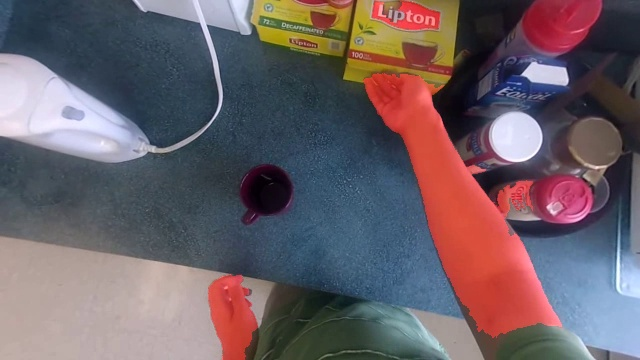
\includegraphics[width=.45\columnwidth]{./Figures/context-free2.jpg}
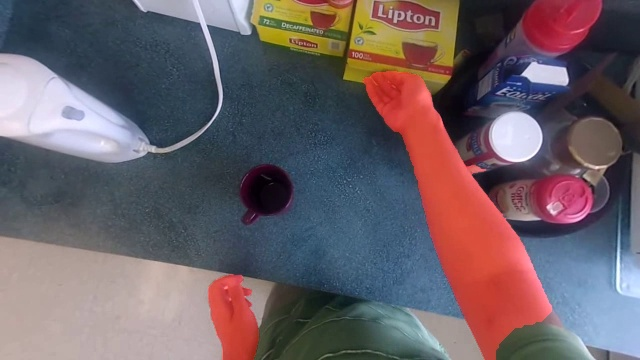
\includegraphics[width=.45\columnwidth]{./Figures/context-dependent2.jpg}
\caption{Comparison before (left image) and after (right image) Temporal smoothing.}
\label{fig:gesture_samples_time}
\end{figure}
We exploit temporal coherence to improve the foreground prediction of a pixel in a frame by a weighted combination of
its previous frames, since past frames should affect the results prediction for the current frame.

The smoothing filter for a pixel $\mathbf{x}_{t}^{i}$ of a frame $t$ (inspired by \cite{liu08}) can thus be defined as follows:

\begin{multline}
P(\mathbf{x}_{t}^{i}=1) = \sum_{k = 0}^{d} w_{k} \bigl( P(\mathbf{x}_{t}^{i}=1|\mathbf{x}_{t-k}^{i}=1) \cdot P(\mathbf{x}_{t-k}^{i}=1|\mathbf{l_{t-k}},\mathbf{g_{t-k}})\, + P(\mathbf{x}_{t}^{i}=1|\mathbf{x}_{t-k}^{i}=0) \, \cdot \\
\cdot P(\mathbf{x}_{t-k}^{i}=0|\mathbf{l_{t-k}},\mathbf{g_{t-k}}) \bigr)
\end{multline}
where $P(\mathbf{x}_{t-k}^{i}=1|\mathbf{l_{t-k}},\mathbf{g_{t-k}})$ is the posterior probability
that a pixel in frame $t-k$ is marked as hand part and $d$ is a number of past frames used. This likelihood can be defined as the probability $P(\mathbf{s}|\mathbf{l_{t-k}},\mathbf{g_{t-k}})$, being
$\mathbf{x}_{t}^{i}$ part of $\mathbf{s}$. In the same way, $P(\mathbf{x}_{t-k}^{i}=0|\mathbf{l_{t-k}},\mathbf{g_{t-k}})$ is defined as the probability
$1-P(\mathbf{s}|\mathbf{l},\mathbf{g_{t-k}})$. 

While $P(\mathbf{x}_{t}^{i}=1|\mathbf{x}_{t-k}^{i}=1)$ and $P(\mathbf{x}_{t}^{i}=1|\mathbf{x}_{t-k}^{i}=0)$ are prior probabilities estimated
from the training set as follows:

\[
P(\mathbf{x}_{t}^{i}=1|\mathbf{x}_{t-k}^{i}=1)=\frac{\#(\mathbf{x}_{t}^{i}=1,\mathbf{x}_{t-k}^{i}=1)}{\#(\mathbf{x}_{t-k}^{i}=1)}
\]


\[
P(\mathbf{x}_{t}^{i}=1|\mathbf{x}_{t-k}^{i}=0)=\frac{\#(\mathbf{x}_{t}^{i}=1,\mathbf{x}_{t-k}^{i}=0)}{\#(\mathbf{x}_{t-k}^{i}=0)}
\]


where $\#(\mathbf{x}_{t-k}^{i}=1)$ and $\#(\mathbf{x}_{t-k}^{i}=0)$ are the number of times in which $\mathbf{x}_{t-k}$ belongs or not to
a hand region, respectively; $\#(\mathbf{x}_{t}^{i}=1,\mathbf{x}_{t-k}^{i}=1)$ is the number
of times that two pixels at the same location at frame $t$ and $t-k$ belong to a hand part; 
similarly, $\#(\mathbf{x}_{t}^{i}=1,\mathbf{x}_{t-k}^{i}=0)$
is the number of times that a pixel in frame $t$ belongs to
a hand part and pixel in the same position in frame $t-k$ does not belong
to a hand region.
Figure \ref{fig:gesture_samples_time} shows an example where temporal smoothing deletes blinking regions (i.e. the tea box brand and jar shadows on the right).


\subsubsection{Spatial consistency}
\begin{figure}[tb]
\centering
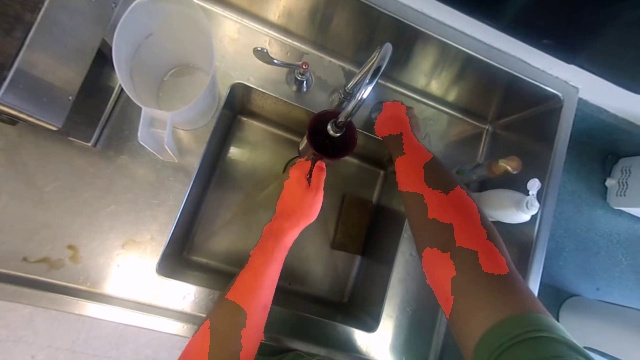
\includegraphics[width=.45\columnwidth]{./Figures/context-free1.jpg}
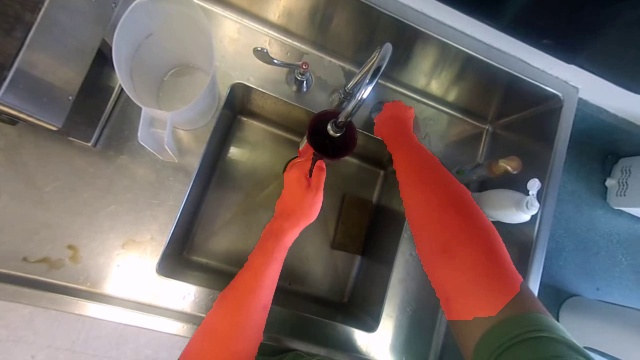
\includegraphics[width=.45\columnwidth]{./Figures/context-dependent1.jpg}
\caption{Comparison before (left image) and after (right image) Spatial Consistency.}
\label{fig:gesture_samples_space}
\end{figure}
Given pixels elaborated by the previous steps, we want to exploit spatial consistency to prune away small and isolated pixel groups that are unlikely to be part of hand regions and also aggregate bigger connected pixel groups. 

For every pixel $\mathbf{x}$, we extract its posterior probability $P(\mathbf{x}_{t}^{i})$ and use it as input for the GrabCut algorithm \cite{rother04}. Each pixel with $P(\mathbf{x}_{t}^{i}) \geq 0.5$ is marked as foreground, otherwise it's considered as part of background. After the segmentation step, we discard all the small isolated regions that have an area of less than 5\% of the frame and we keep only the three largest connected components.

In Figure \ref{fig:gesture_samples_space} an example with and without applying the Spatial Consistency method is depicted; notice this technique allows to better aggregate superpixels that are near the principal blob region.


\begin{figure*}[tb]
\centering
\subfigure[]{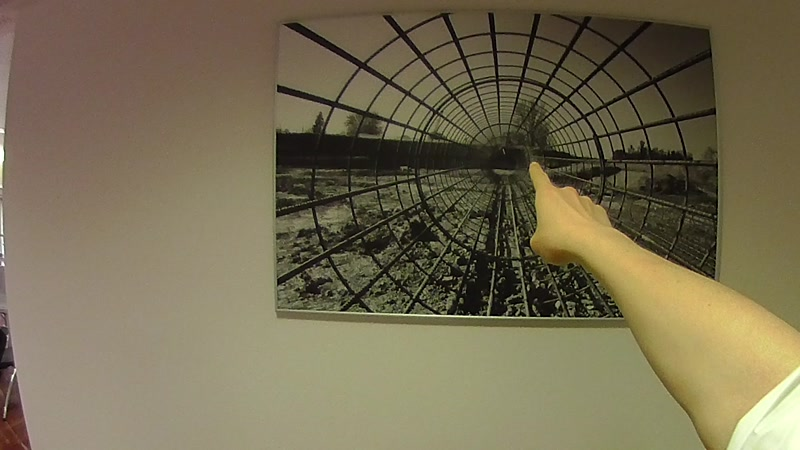
\includegraphics[width=.30\columnwidth]{./Figures/index_sample.jpg}}
\subfigure[]{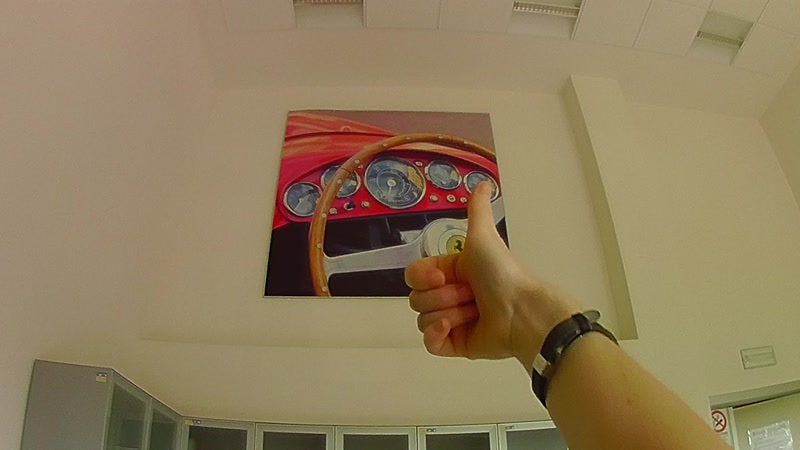
\includegraphics[width=.30\columnwidth]{./Figures/like_sample.jpg}}
\subfigure[]{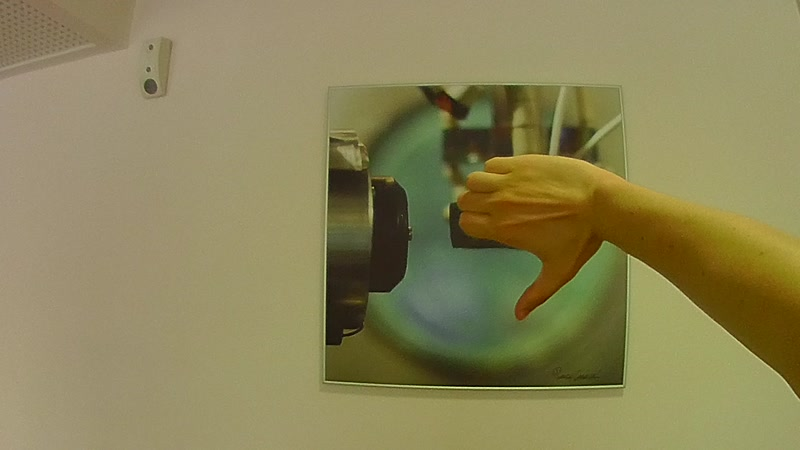
\includegraphics[width=.30\columnwidth]{./Figures/dislike_sample.jpg}}
\subfigure[]{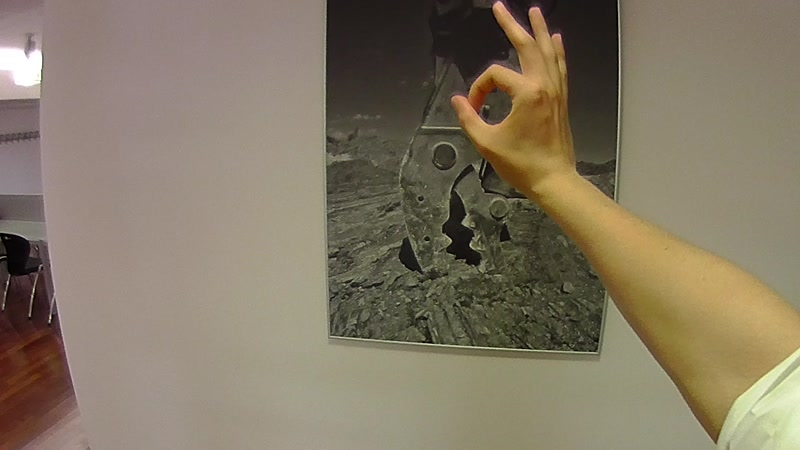
\includegraphics[width=.30\columnwidth]{./Figures/ok_sample.jpg}}
\subfigure[]{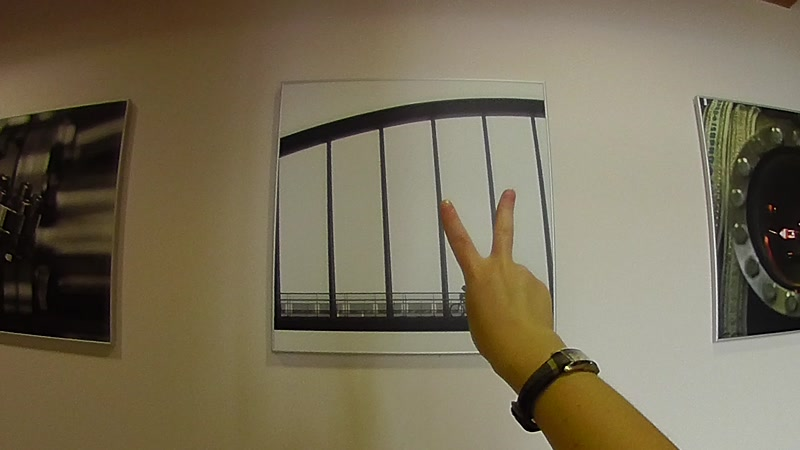
\includegraphics[width=.30\columnwidth]{./Figures/victory_sample.jpg}}
\caption{Our dataset consists of five gestures: a) point out; b) like; c) dislike; d) ok; e) victory.}
\label{fig:gesture_samples}
\end{figure*}

\section{Experimental results}
To evaluate the performance of proposed method we tested it on two datasets: EDSH and EGO-HSGR.
The recent publicly available EDSH dataset \cite{li13} consists in egocentric videos acquired to analyze performance of several hand detection methods. It consists in three videos (EDSH\_1, used as train video, and EDSH\_2 and EDSH\_{kitchen} used as test videos) that contain indoor and outdoor scenes with large variations of illumination, mild camera motion induced by walking and climbing stairs. All videos are recorded at a resolution of 720p and a speed of 30FPS. The dataset includes segmentation masks of hands, but it is not comprehensive of gesture annotations.     


In order to analyze the performance of our method to recognize gestures, we generated a new dataset which contains 12 videos of indoor scenes (EGO-HSGR); it includes segmentation masks and gesture annotations. Videos have been recorded with a Panasonic HX-A10 Wearable Camcorder at a resolution of $800 \times 450$ with a 25FPS in two different locations: a library and department's exhibition area.   

The aim of this dataset is to reproduce an environment similar to a museum for human and object interaction: paintings and posters are hung on the walls, true masterpieces or either its virtual images; the visitor walks and sometimes stops in front of an object of interest performing some gestures to interact with next generation wearable devices. We identify five different gestures that are used commonly: \textit{point out}, \textit{like}, \textit{dislike}, \textit{ok} and \textit{victory}. These can be associated to different action or used for record social experience. Fig. \ref{fig:gesture_samples} shows some frame examples. 

To evaluate performance of our pixel-level hand detector a subset of six videos are used (three for training and two for testing). Segmentation masks are provided every 25 frames for a total of 700 annotations. For gesture analysis we extract all the keyframes and we manually annotated them distinguishing between gestures.  
The F-score (harmonic mean of the precision and recall rate) is used to quantity hand detection performance, while gesture recognition is evaluated in terms of mAP (mean Average Precision).
%(we denote these videos as BB\_L1 and BB\_L2), a corridor of a faculty (BB\_F1 and BB\_F2) and a department (BB\_D1 and BB\_D2).
    
 \begin{table}
 \centering
 \begin{tabular}{|l|c|c|}
 \hline
 \textbf{Features} 	& \textbf{EDSH\_2} & \textbf{EDSH\_{kitchen}}	\\ \hline\hline
 HSV	& 0.752 & 0.801		\\ \hline
 + LAB	& 0.754	&	0.808 \\ \hline
 + LAB hist.	& 0.755 & 0.823			\\ \hline  
 + HSV hist. & 0.755 & 0.823			\\ \hline  
 + Grad hist. & 0.758	&	0.828	\\ \hline  
 + Gabor & 	\textbf{0.761}	& \textbf{0.829} \\ \hline  
 \end{tabular}
 \caption{Performance by incrementally adding new features.}\label{tab:localfeatures}
 \end{table}

\subsection{Features performance}

First, we examine the effectiveness of our features to discriminate between hand and non-hand superpixels. 
Table \ref{tab:localfeatures} shows performance in terms of F-measure on EDSH dataset with different feature combinations: firstly we describe each superpixel with mean and covariance matrix of its pixel values in HSV color space, then we do the same using LAB color space and we add color histograms. Lastly, we include a histogram of gradients and Gabor feature.
In order to analyze how visual features impact on the performance, in this experiment we do not include the temporal and spatial context information by using a single random forest classifier.     
Note that although color information plays a fundamental role for hand detection, some ambiguities between hands and other similar colored object still remain; these can be reduced by adding features based on gradient histograms. In fact, the usage of the full descriptor slightly improves the performance.      

\begin{table}
 \centering
 \begin{tabular}{|l|c|c|}
 \hline
 \textbf{Features} 	& \textbf{EDSH\_2} & \textbf{EDSH\_{kitchen}}	\\ \hline\hline
 II	& 0.789 & 	0.831		\\ \hline
 II + TS	& 0.791	&	0.834 \\ \hline
 II + TS + SC &	\textbf{0.852} &	\textbf{0.901}	\\ \hline  
 \end{tabular}
 \caption{Performance comparison considering Illumination Invariance (II), Time Smoothing (TS) and Spatial Consistency (SC).}\label{tab:context}
\end{table}


\subsection{Temporal Smoothing and Spatial Consistency}
In this experiment we validate the proposed techniques that take into account illumination variations, time dependence and spatial consistency.
Table \ref{tab:context} shows the F-measure scores obtained on EDSH dataset incrementally adding Illumination Invariance (II), Time Smoothing (TS) and Spatial Consistency (SC). 
Note that there is a significant improvement in performance when all these three techniques are applied together.   
In particular, illumination invariance substantially increases the performance with respect to results obtained using only visual features and a single random forest classifier, while the improvement introduced by temporal smoothing is less pronounced. The main contribution is given by Spatial Consistency, that prunes away small and isolated pixel groups and merge spatially nearby regions, increasing the F-measure score of about six percentage points.
The proposed technique is also tested in our EGO-HSGR dataset obtaining an F-measure score of $0.908$ and $0.865$ for the EGO-HSGR\_{4} and EGO-HSGR\_{5} videos.        


\begin{table}
 \centering
 \begin{tabular}{|l|c|c|}
 \hline
  	& \textbf{EDSH\_2}	& \textbf{EDSH\_{kitchen}} \\ \hline\hline
Hayman \etal \cite{hayman03} 	& 0.211 & 0.213		\\ \hline
Jones \etal \cite{jones99}	& 0.708 &	0.787	\\ \hline  
Li \etal \cite{li13} & 0.835 & 0.840		\\ \hline  
\textbf{Our method} & \textbf{0.852} &	\textbf{0.901}	\\ \hline 
\end{tabular}
\caption{Hand segmentation comparison with the state-of-the-art.}\label{tab:comparision_hand}
\end{table}



\subsection{Comparison to related methods}

In Table \ref{tab:comparision_hand} we compare our results to several approaches on EDSH dataset: a single-pixel color approach inspired by \cite{jones99}, a video stabilization approach based on background modeling using affine alignment of image frames inspired by
\cite{hayman03} and an approach based on random forest, proposed by \cite{li13}. 
The single-pixel approach is a random regressor trained only using single-pixel LAB color values. 
The background modeling approach aligns sequences of 15 frames estimating their mutual affine transformations; pixels with high variance are considered to be foreground hand regions. 
As can be seen, although the single-pixel approach is conceptually simple, is still quite effective. In addition, we observe that the low performance of the video stabilization approach is due to large ego-motion because the camera is worn by the user.     
The method recently proposed by \cite{li13} is more similar to our approach, but the use of superpixels, the selection of a new set of local features and the introduction of temporal and spatial consistency allow us to outperforms that results.
